\documentclass[12pt]{article}

% Layout.
\usepackage[top=1in, bottom=0.75in, left=1in, right=1in, headheight=1in, headsep=6pt]{geometry}

% Fonts.
\usepackage{mathptmx}
\usepackage[scaled=0.86]{helvet}
\renewcommand{\emph}[1]{\textsf{\textbf{#1}}}

% TiKZ.
\usepackage{tikz, pgfplots}

\usetikzlibrary{calc,trees,positioning,arrows,fit,shapes,through, backgrounds}
\usetikzlibrary{patterns}

\usetikzlibrary{decorations.markings}
\usetikzlibrary{arrows}

\usepackage{pgfplots}


% Misc packages.
\usepackage{amsmath,amssymb,latexsym}
\usepackage{graphicx}
\usepackage{array}
\usepackage{xcolor}
\usepackage{multicol}
\usepackage{fancyhdr}
\pagestyle{fancy}


% Misc.
\renewcommand{\d}{\displaystyle}
\newcommand{\ds}{\displaystyle}
\newcommand{\ul}[1]{\underline{#1}}
\def\bc{\begin{center}}
\def\ec{\end{center}}
\def\be{\begin{enumerate}}
\def\ee{\end{enumerate}}

\newcommand{\ans}[1][1in]{\rule{#1}{.5pt}}


\lhead{Math F113X: Quiz 4}
\rhead{October 10, 2025}

\begin{document}

\vspace{1cm}
\strut

\noindent \textbf{Name:} \hrulefill \quad  score:\ans[1cm] \ / 10 \\


\noindent There are 10 points possible on this quiz. No aids (book, notes, etc.)
are permitted. You may use a calculator.  {\bf Show all work and supporting calculations for full credit. Explain how you get your answers.}



\be

\item (2 points) Describe a situation that can be modeled with a \emph{weighted} graph.% What do the vertices represent? What do the edges represent? What do the weights represent?

What do the \emph{vertices} represent?

\vfill

What do the \emph{edges} represent? 

\vfill

What do the \emph{weights} represent?

\vfill


\item (4 points) Consider the following graph:

\makeatletter
\newcommand{\Letter}[1]{\@Alph{#1}}
\makeatother

\begin{center}
\begin{tikzpicture}[baseline=(current bounding box.center),vertex/.style = {circle, draw, inner sep=2pt}]

\foreach \i in {1,...,5}{\node[vertex] (\Letter{\i}) at (360*\i/5:2) {\Letter{\i}};}
\node[vertex, right = of E] (F) {F};
\node[vertex, right = 3 cm of E] (G) {G};
\foreach \i/\j in {A/D, D/F, A/F, B/C, C/E, E/B}{\draw (\i) -- (\j);}
\draw (E) edge[bend left = 30] (G);
\draw (E) edge[bend right = 30] (G);
\end{tikzpicture}
\end{center}

\be
\item How many vertices does this graph have? \ans
\item How many edges does this graph have? \ans
\item What is the degree of vertex $E$? \ans
\item Explain why this graph is not connected.

\vspace{1in}
\ee

	\newpage
	
	\item (4 points) Recall Kruskal's algorithm roughly says the following:
	
	\fbox{Kruskal's Algorithm} Select the cheapest edge in the graph that does not create a circuit. Stop when a spanning tree is obtained.\\

Use Kruskal's Algorithm to find a minimum weight spanning tree in the graph below. Break ties by choosing the alphabetically earliest edge first.

%Draw your spanning tree on the empty copy of the graph.

\bigskip
\bigskip


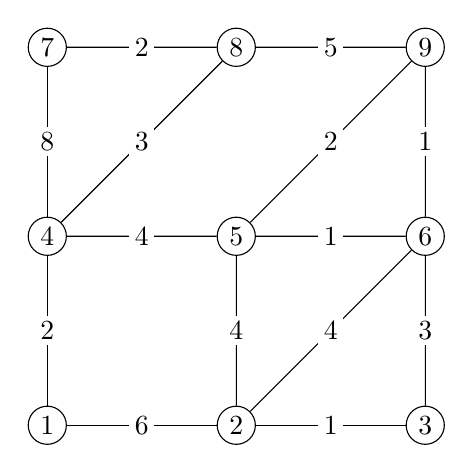
\begin{tikzpicture}[baseline=(current bounding box.center),lbl/.style={fill=white, inner sep = 2pt, }, scale = 1.2]
\tikzstyle{vtx}=[circle, draw, inner sep=2pt]%, minimum size=6pt]
\foreach \i in {0,1,2}{
\path let \n1 = {int(\i+0)}, \n2 = {int(\i+0+1)} in node[vtx] (v\n1) at (2*\i,2*0){$\Letter{\n2}$};
\path let \n1 = {int(\i+3)},\n2 = {int(\i+3+1)} in node[vtx] (v\n1) at (2*\i,2*1){$\Letter{\n2}$};
\path let \n1 = {int(\i+6)},\n2 = {int(\i+6+1)} in node[vtx] (v\n1) at (2*\i,2*2){$\Letter{\n2}$};
 }
 
% \path (v0) node[vtx, ultra thick] {$V_{0}$};
%  \path  (v8) node[vtx, ultra thick]{$V_{8}$};


\foreach \i/\j/\k in {0/1/6, 1/2/1, 0/3/2, 1/4/4, 1/5/4, 2/5/3, 3/4/4, 4/5/1, 5/8/1, 4/8/2, 3/7/3, 3/6/8, 6/7/2, 7/8/5}{
\draw (v\i) --node[lbl]{\k} (v\j);
}


\end{tikzpicture}
%%
\hfill
\begin{tabular} {p{1.5cm}|c | c}
used? & edges  & weights \\ \hline \hline
&BC & 1\\ \hline
&EF & 1\\ \hline
&FI & 1\\ \hline
&AD & 2\\ \hline
&EI & 2\\ \hline
&GH & 2\\ \hline
&CF & 3\\ \hline
&DH & 3\\ \hline
&BE & 4\\ \hline
&BF & 4\\ \hline
&DE & 4\\ \hline
&HI & 5\\ \hline
&AB & 6\\ \hline
&DG & 8
\end{tabular}

Draw the minimum weight spanning tree below. 

\vfill

%%
\begin{tikzpicture}[baseline=(current bounding box.center),lbl/.style={fill=white, inner sep = 2pt, }, scale = 1.2]
\tikzstyle{vtx}=[circle, draw, inner sep=2pt]%, minimum size=6pt]
\foreach \i in {0,1,2}{
\path let \n1 = {int(\i+0)}, \n2 = {int(\i+0+1)} in node[vtx] (v\n1) at (2*\i,2*0){$\Letter{\n2}$};
\path let \n1 = {int(\i+3)},\n2 = {int(\i+3+1)} in node[vtx] (v\n1) at (2*\i,2*1){$\Letter{\n2}$};
\path let \n1 = {int(\i+6)},\n2 = {int(\i+6+1)} in node[vtx] (v\n1) at (2*\i,2*2){$\Letter{\n2}$};
 }
 
% \path (v0) node[vtx, ultra thick] {$V_{0}$};
%  \path  (v8) node[vtx, ultra thick]{$V_{8}$};


%\foreach \i/\j/\k in {0/1/2, 0/3/5, 1/2/3, 2/5/1, 3/4/6, 4/5/2, 1/4/5, 3/6/7, 3/7/2,  4/8/9, 5/8/3, 6/7/2, 7/8/1, 1/5/6}{
%\draw (v\i) --node[lbl]{\k} (v\j);
%}

\end{tikzpicture}

\bigskip

\bigskip


What is the total weight of the spanning tree you found? \ans
	
	\vfill
	

 \ee
\end{document}